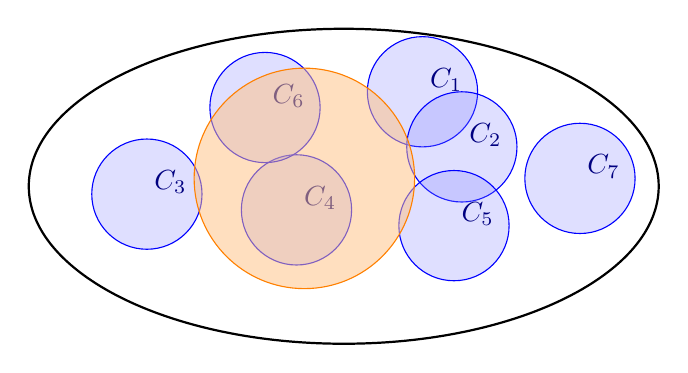
\begin{tikzpicture}
    \def\r{0.7}
    \def\vars{(1, 1.2), (1.5, 0.5), (-2.5, -0.1), (-0.6, -0.3), (1.4, -0.5), (-1, 1), (3, 0.1)}
    
    \draw[thick] (0, 0) ellipse (4 and 2);

    \foreach \a  [count = \i] in \vars{
        \draw[blue, fill = blue!50, fill opacity = 0.25] \a circle (0.7) ++(0.3, 0.15)
            node[opacity = 1, blue!50!black] {$C_{\i}$};
    }
        
    \only<3->{
        \draw[orange, fill = orange!50, fill opacity = 0.5] (-0.5, 0.1) circle (1.4)
            ++(0.5, 0.5);% node[orange!50!black, opacity = 1] {$W$};
    }
        
\end{tikzpicture}